% This file was created with matplot2tikz v0.5.3.
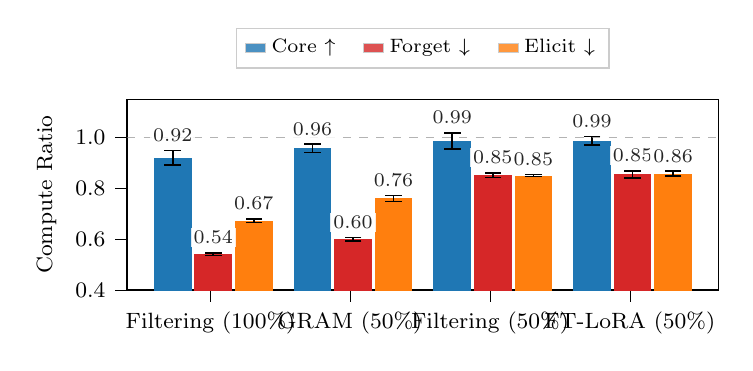
\begin{tikzpicture}

\pgfplotsset{legend image code/.code={\draw[#1] (0cm,-0.06cm) rectangle (0.25cm,0.06cm);}}

\definecolor{crimson2143940}{RGB}{214,39,40}
\definecolor{darkgray176}{RGB}{176,176,176}
\definecolor{darkorange25512714}{RGB}{255,127,14}
\definecolor{gray}{RGB}{128,128,128}
\definecolor{lightgray204}{RGB}{204,204,204}
\definecolor{steelblue31119180}{RGB}{31,119,180}

\begin{axis}[
scale only axis=true,
tick label style={font=\footnotesize},
label style={font=\footnotesize},
height=0.20\linewidth,
legend cell align={left},
legend columns=3,
legend style={
  font=\scriptsize,
  /tikz/every even column/.append style={column sep=8pt},
  fill opacity=0.8,
  draw opacity=1,
  text opacity=1,
  at={(0.5,1.16)},
  anchor=south,
  draw=lightgray204
},
tick align=outside,
tick pos=left,
width=0.62\linewidth,
x grid style={darkgray176},
xmin=-0.5975, xmax=3.6375,
xtick style={color=black},
xtick={0,1,2,3},
xticklabels={Filtering (100\%),GRAM (50\%),Filtering (50\%),FT-LoRA (50\%)},
y grid style={darkgray176},
ylabel={Compute Ratio},
ymin=0.4, ymax=1.15,
ytick={0.4,0.6,0.8,1},
yticklabels={0.4,0.6,0.8,1.0},
ytick style={color=black}
]
\draw[draw=none,fill=steelblue31119180] (axis cs:-0.405,0) rectangle (axis cs:-0.135,0.919816453392059);
\addlegendimage{draw=none,fill=steelblue31119180}
\addlegendentry{Core $\uparrow$}

\draw[draw=none,fill=steelblue31119180] (axis cs:0.595,0) rectangle (axis cs:0.865,0.956554500091221);
\draw[draw=none,fill=steelblue31119180] (axis cs:1.595,0) rectangle (axis cs:1.865,0.985642892899399);
\draw[draw=none,fill=steelblue31119180] (axis cs:2.595,0) rectangle (axis cs:2.865,0.985569865596572);
\draw[draw=none,fill=crimson2143940] (axis cs:-0.115,0) rectangle (axis cs:0.155,0.540553550804861);
\addlegendimage{draw=none,fill=crimson2143940}
\addlegendentry{Forget $\downarrow$}

\draw[draw=none,fill=crimson2143940] (axis cs:0.885,0) rectangle (axis cs:1.155,0.599643902402252);
\draw[draw=none,fill=crimson2143940] (axis cs:1.885,0) rectangle (axis cs:2.155,0.85103331203406);
\draw[draw=none,fill=crimson2143940] (axis cs:2.885,0) rectangle (axis cs:3.155,0.854250433220036);
\draw[draw=none,fill=darkorange25512714] (axis cs:0.175,0) rectangle (axis cs:0.445,0.672466580236959);
\addlegendimage{draw=none,fill=darkorange25512714}
\addlegendentry{Elicit $\downarrow$}

\draw[draw=none,fill=darkorange25512714] (axis cs:1.175,0) rectangle (axis cs:1.445,0.759859199958449);
\draw[draw=none,fill=darkorange25512714] (axis cs:2.175,0) rectangle (axis cs:2.445,0.849548915544174);
\draw[draw=none,fill=darkorange25512714] (axis cs:3.175,0) rectangle (axis cs:3.445,0.856652078327302);
\path [draw=black, semithick]
(axis cs:-0.27,0.891003780865332)
--(axis cs:-0.27,0.948629125918786);

\path [draw=black, semithick]
(axis cs:0.73,0.940757548636747)
--(axis cs:0.73,0.972351451545694);

\path [draw=black, semithick]
(axis cs:1.73,0.954557085959313)
--(axis cs:1.73,1.01672869983948);

\path [draw=black, semithick]
(axis cs:2.73,0.968778832280486)
--(axis cs:2.73,1.00236089891266);

\addplot [semithick, steelblue31119180, mark=-, mark size=3, mark options={solid,draw=black}, only marks]
table {%
-0.27 0.891003780865332
0.73 0.940757548636747
1.73 0.954557085959313
2.73 0.968778832280486
};
\addplot [semithick, steelblue31119180, mark=-, mark size=3, mark options={solid,draw=black}, only marks]
table {%
-0.27 0.948629125918786
0.73 0.972351451545694
1.73 1.01672869983948
2.73 1.00236089891266
};
\path [draw=black, semithick]
(axis cs:0.02,0.535372404880425)
--(axis cs:0.02,0.545734696729297);

\path [draw=black, semithick]
(axis cs:1.02,0.593220213518262)
--(axis cs:1.02,0.606067591286241);

\path [draw=black, semithick]
(axis cs:2.02,0.841536152825519)
--(axis cs:2.02,0.860530471242601);

\path [draw=black, semithick]
(axis cs:3.02,0.840945107944566)
--(axis cs:3.02,0.867555758495506);

\addplot [semithick, steelblue31119180, mark=-, mark size=3, mark options={solid,draw=black}, only marks]
table {%
0.02 0.535372404880425
1.02 0.593220213518262
2.02 0.841536152825519
3.02 0.840945107944566
};
\addplot [semithick, steelblue31119180, mark=-, mark size=3, mark options={solid,draw=black}, only marks]
table {%
0.02 0.545734696729297
1.02 0.606067591286241
2.02 0.860530471242601
3.02 0.867555758495506
};
\path [draw=black, semithick]
(axis cs:0.31,0.664738070976287)
--(axis cs:0.31,0.680195089497632);

\path [draw=black, semithick]
(axis cs:1.31,0.748116482763705)
--(axis cs:1.31,0.771601917153194);

\path [draw=black, semithick]
(axis cs:2.31,0.845431720677439)
--(axis cs:2.31,0.853666110410909);

\path [draw=black, semithick]
(axis cs:3.31,0.847095513442829)
--(axis cs:3.31,0.866208643211775);

\addplot [semithick, steelblue31119180, mark=-, mark size=3, mark options={solid,draw=black}, only marks]
table {%
0.31 0.664738070976287
1.31 0.748116482763705
2.31 0.845431720677439
3.31 0.847095513442829
};
\addplot [semithick, steelblue31119180, mark=-, mark size=3, mark options={solid,draw=black}, only marks]
table {%
0.31 0.680195089497632
1.31 0.771601917153194
2.31 0.853666110410909
3.31 0.866208643211775
};
\addplot [line width=0.28pt, gray, opacity=0.6, dashed, forget plot]
table {%
-0.5975 1
3.6375 1
};
\draw (axis cs:-0.27,0.969980428615415) node[
  font=\scriptsize,
  fill=white,
  draw=none,
  line width=0.4pt,
  inner sep=1.1pt,
  fill opacity=0.85,
  anchor=south,
  text=black,
  rotate=0.0
]{0.92};
\draw (axis cs:0.73,0.993702754242324) node[
  font=\scriptsize,
  fill=white,
  draw=none,
  line width=0.4pt,
  inner sep=1.1pt,
  fill opacity=0.85,
  anchor=south,
  text=black,
  rotate=0.0
]{0.96};
\draw (axis cs:1.73,1.03808000253611) node[
  font=\scriptsize,
  fill=white,
  draw=none,
  line width=0.4pt,
  inner sep=1.1pt,
  fill opacity=0.85,
  anchor=south,
  text=black,
  rotate=0.0
]{0.99};
\draw (axis cs:2.73,1.02371220160929) node[
  font=\scriptsize,
  fill=white,
  draw=none,
  line width=0.4pt,
  inner sep=1.1pt,
  fill opacity=0.85,
  anchor=south,
  text=black,
  rotate=0.0
]{0.99};
\draw (axis cs:0.02,0.567085999425926) node[
  font=\scriptsize,
  fill=white,
  draw=none,
  line width=0.4pt,
  inner sep=1.1pt,
  fill opacity=0.85,
  anchor=south,
  text=black,
  rotate=0.0
]{0.54};
\draw (axis cs:1.02,0.62741889398287) node[
  font=\scriptsize,
  fill=white,
  draw=none,
  line width=0.4pt,
  inner sep=1.1pt,
  fill opacity=0.85,
  anchor=south,
  text=black,
  rotate=0.0
]{0.60};
\draw (axis cs:2.02,0.88188177393923) node[
  font=\scriptsize,
  fill=white,
  draw=none,
  line width=0.4pt,
  inner sep=1.1pt,
  fill opacity=0.85,
  anchor=south,
  text=black,
  rotate=0.0
]{0.85};
\draw (axis cs:3.02,0.888907061192135) node[
  font=\scriptsize,
  fill=white,
  draw=none,
  line width=0.4pt,
  inner sep=1.1pt,
  fill opacity=0.85,
  anchor=south,
  text=black,
  rotate=0.0
]{0.85};
\draw (axis cs:0.31,0.701546392194261) node[
  font=\scriptsize,
  fill=white,
  draw=none,
  line width=0.4pt,
  inner sep=1.1pt,
  fill opacity=0.85,
  anchor=south,
  text=black,
  rotate=0.0
]{0.67};
\draw (axis cs:1.31,0.792953219849823) node[
  font=\scriptsize,
  fill=white,
  draw=none,
  line width=0.4pt,
  inner sep=1.1pt,
  fill opacity=0.85,
  anchor=south,
  text=black,
  rotate=0.0
]{0.76};
\draw (axis cs:2.31,0.875017413107538) node[
  font=\scriptsize,
  fill=white,
  draw=none,
  line width=0.4pt,
  inner sep=1.1pt,
  fill opacity=0.85,
  anchor=south,
  text=black,
  rotate=0.0
]{0.85};
\draw (axis cs:3.31,0.887559945908404) node[
  font=\scriptsize,
  fill=white,
  draw=none,
  line width=0.4pt,
  inner sep=1.1pt,
  fill opacity=0.85,
  anchor=south,
  text=black,
  rotate=0.0
]{0.86};
\end{axis}

\end{tikzpicture}
